\chapter{Model Architecture and Experiments}
\phantomsection
\label{ch:experiments}


\section{End-to-End Khmer OCR Network system}
\label{sec:end_to_end_khmer_ocr_sysetm}

We propose an end-to-end Khmer OCR pipeline that combines the CRAFT model 
for text detection with the TrOCR model architecture developed by Microsoft 
for text recognition. We have customized and adapted the system to support 
both Khmer and English languages. The pipeline takes an input image, applies 
the CRAFT model to detect and crop individual text-line regions, and then 
feeds each text-line image into the TrOCR model.
The TrOCR model operates in an auto-regressive manner, decoding one character 
at a time until it reaches the end-of-sequence token. This approach allows the 
system to handle variable-length input text-lines without any predefined limit, 
as long as the input fits within the model’s maximum token capacity.
This is a high-level description of the system architecture. Importantly, 
our pipeline operates without any preprocessing steps like binarization, 
noise removal, or skew adjustment. It processes raw input images directly, 
handling both detection and recognition seamlessly within a unified end-to-end 
framework.

\begin{figure}[H]
    \centering
    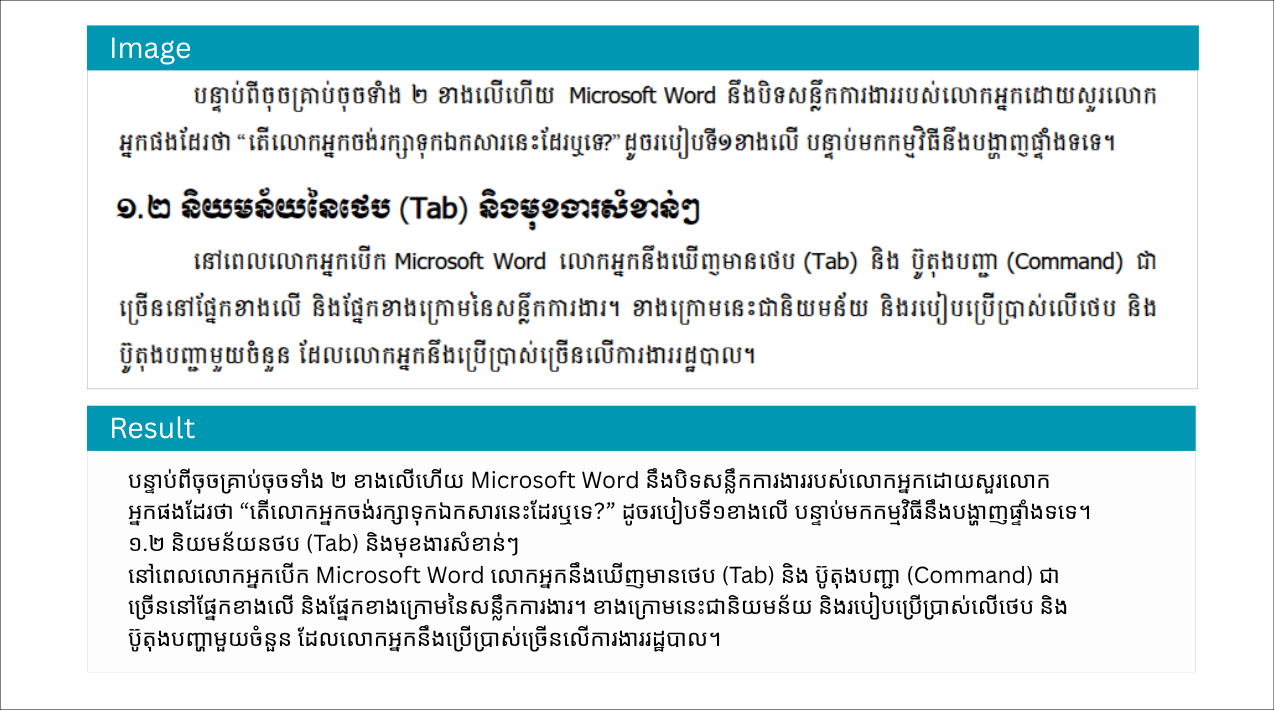
\includegraphics[width=\textwidth]{figures/result_image_to_text.png}
    \caption{End-to-end OCR result: The pipeline takes a raw image as input 
    and outputs recognized text directly without any manual preprocessing.}
    \label{fig:result_converted}
\end{figure}

\section{Experimental Environment and Tools}
\label{sec:environment}

All experiments were conducted on a Linux CLI system with the following hardware
and software specifications listed below:

\begin{table}[H]
    \centering
    \caption{Experimental Setup and Environment Configuration}
    \renewcommand{\arraystretch}{1.4}
    \resizebox{\textwidth}{!}{%
    \begin{tabular}{|p{4.5cm}|p{5.7cm}|p{6.5cm}|}
    \hline
    \textbf{Component} & \textbf{Specification} & \textbf{Purpose} \\[0.2cm]
    \hline
    \multicolumn{3}{|c|}{\textbf{Hardware Configuration}} \\[0.2cm]
    \hline
    Operating System & Ubuntu 20.04 LTS & Stable training large model \\[0.2cm]
    \hline
    GPU Units & 3x NVIDIA RTX 4090 & Parallel computing \\[0.2cm]
    \hline
    VRAM & 24 GB per GPU (72 GB total) & Large model training and inference \\[0.2cm]
    \hline
    System Memory & 256 GB RAM & Great for loading \& processing \\[0.2cm]
    \hline
    \multicolumn{3}{|c|}{\textbf{Software Framework}} \\[0.2cm]
    \hline
    DL Framework & PyTorch & implementation \& training \\[0.2cm]
    \hline
    Model Library & Hugging Face Transformers & Pre-trained architecture access \\[0.2cm]
    \hline
    GPU Acceleration & CUDA & Great for training across GPUs \\[0.2cm]
    \hline
    \multicolumn{3}{|c|}{\textbf{Experiment Management}} \\[0.2cm]
    \hline
    Tracking System & MLflow & Real-time metric logging \\[0.2cm]
    \hline
    Monitored Metrics & CER, Train/Valid Loss & evaluation \& comparison \\[0.2cm]
    \hline
    \end{tabular}%
    }
    \label{tab:experimental_setup}
\end{table}

\section{CRAFT for Text Detection}
\label{sec:craft-complete}

This section presents a comprehensive overview of the CRAFT 
(Character Region Awareness for Text Detection) model implementation, 
covering its architecture, configuration, training methodology, dataset 
preparation, and evaluation metrics.

\subsection{CRAFT Model Architecture}
\label{subsec:craft-architecture}

For the text detection stage, we adopted the Character Region Awareness for Text 
Detection (CRAFT) model, which is a fully convolutional network architecture 
based on VGG-16 with batch normalization is adopted as this architecture's backbone.
The model has skip connections in the decoding part, which is similar to U-net in
that aggregates low-level features. The final output is producing two channels as 
score maps:
\begin{itemize}
\item A \textbf{region score map}, indicating the likelihood of each pixel belonging 
to a character region.
\item An \textbf{affinity score map}, capturing the spatial relationships between 
adjacent characters to form text lines.
\end{itemize}

Unlike traditional text detectors that rely on bounding-box regression, 
CRAFT performs pixel-level predictions to detect the centers of individual 
characters and the affinities between them, allowing it to handle curved, 
rotated, or irregular text effectively. However, in our work, we focus on 
text-line-level detection rather than character-level because Khmer is a 
complex writing system. Many characters are visually dependent, invisible, 
or cannot appear independently, making character-level detection unreliable 
for curved or rotated Khmer text. Since curved text detection relies on accurate 
per-character localization and grouping, CRAFT's character-centric design does 
not perform well on curved Khmer scripts.



\begin{figure}[H]
    \centering
    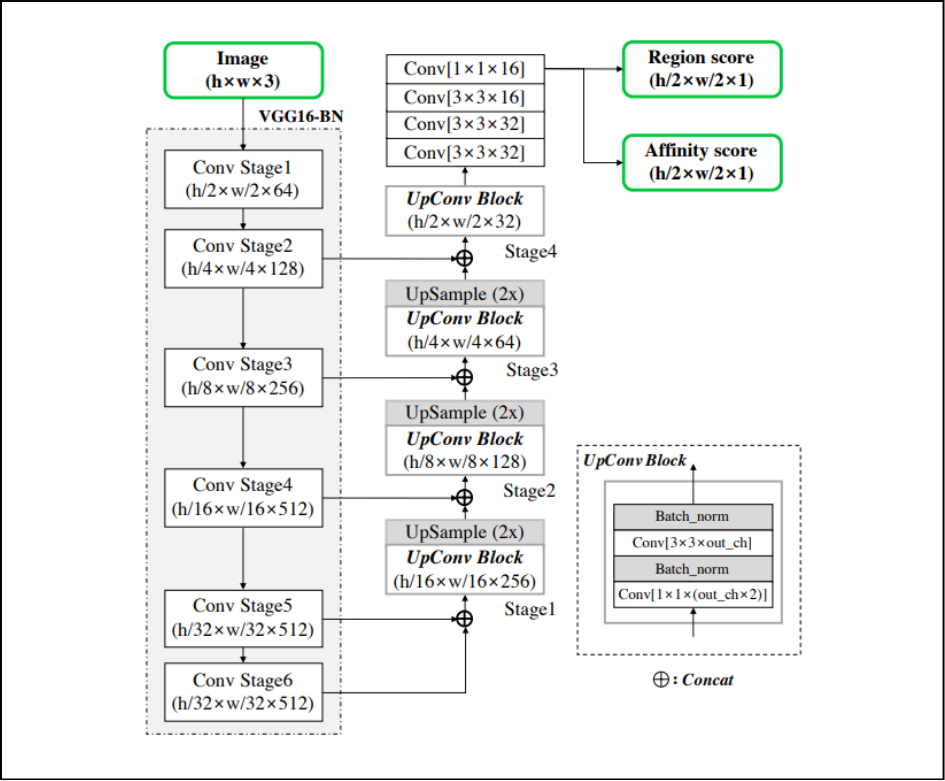
\includegraphics[width=\textwidth]{figures/craft_model.png}
    \caption{Schematic illustration of our CRAFT network architecture.
    \citep{baek2019craft}}
    \label{fig:craft-model}
\end{figure}

The model has 20,770,466 trainable parameters. We used the official 
implementation of CRAFT with some modifications to better support Khmer text. 


\subsection{CRAFT Training Configuration}
\label{subsec:craft-training-config}

The CRAFT model was fine-tuned on a custom Khmer text dataset using weak supervision, leveraging the strengths of annotated real-world images. The key configuration parameters for training the CRAFT model are summarized in Table~\ref{tab:craft-training-config}.

\begin{table}[H]
\centering
\begin{tabular}{|p{0.4\linewidth}|p{0.55\linewidth}|}
\hline
\textbf{Parameter} & \textbf{Value} \\
\hline
Backbone architecture & VGG-16 \\
Pretrained weights & \texttt{CRAFT.pth} \\
Batch size & 8 \\
Training iterations & 0 to 10,000 \\
Evaluation interval & Every 500 iterations \\
Learning rate & 0.0001 \\
Optimizer & Adam \\
Input image size & 768px (height, aspect ratio preserved) \\
\hline
\end{tabular}
\caption{Key configuration parameters for training the CRAFT model on a custom Khmer dataset 
using weak supervision.}
\label{tab:craft-training-config}
\end{table}

\subsection{CRAFT Dataset and Data Augmentation}
\label{subsec:craft-dataset}

Throughout the training process, a variety of data augmentation techniques were employed to enhance the model's robustness against font diversity, image noise, and other real-world distortions. These augmentations included:

\begin{itemize}
\item Random rotation of text instances by up to 20 degrees
\item Random cropping with varying scales and aspect ratios
\item Horizontal flipping to introduce mirrored perspectives
\item Color jittering involving simultaneous adjustments in brightness, contrast, saturation, and hue (each parameter varied by a factor of 0.2)
\end{itemize}

These transformations enriched the training set with diverse visual variations, which helped the model generalize more effectively to unseen examples. We fine-tuned the pretrained model using a manually annotated dataset comprising 4,000 bounding boxes that captured the intricate structure of the Khmer script, including its unique diacritics and ligatures.

\subsection{CRAFT Training Process and Results}
\label{subsec:craft-training-results}

The model was trained using Adam optimizer with early stopping and validation-based checkpointing to prevent overfitting. To further strengthen the model's discriminative capabilities, we incorporated contrastive learning alongside adversarial training, which were particularly beneficial in enabling the model to distinguish between visually similar Khmer characters and different font styles.

\begin{figure}[H]
    \centering
    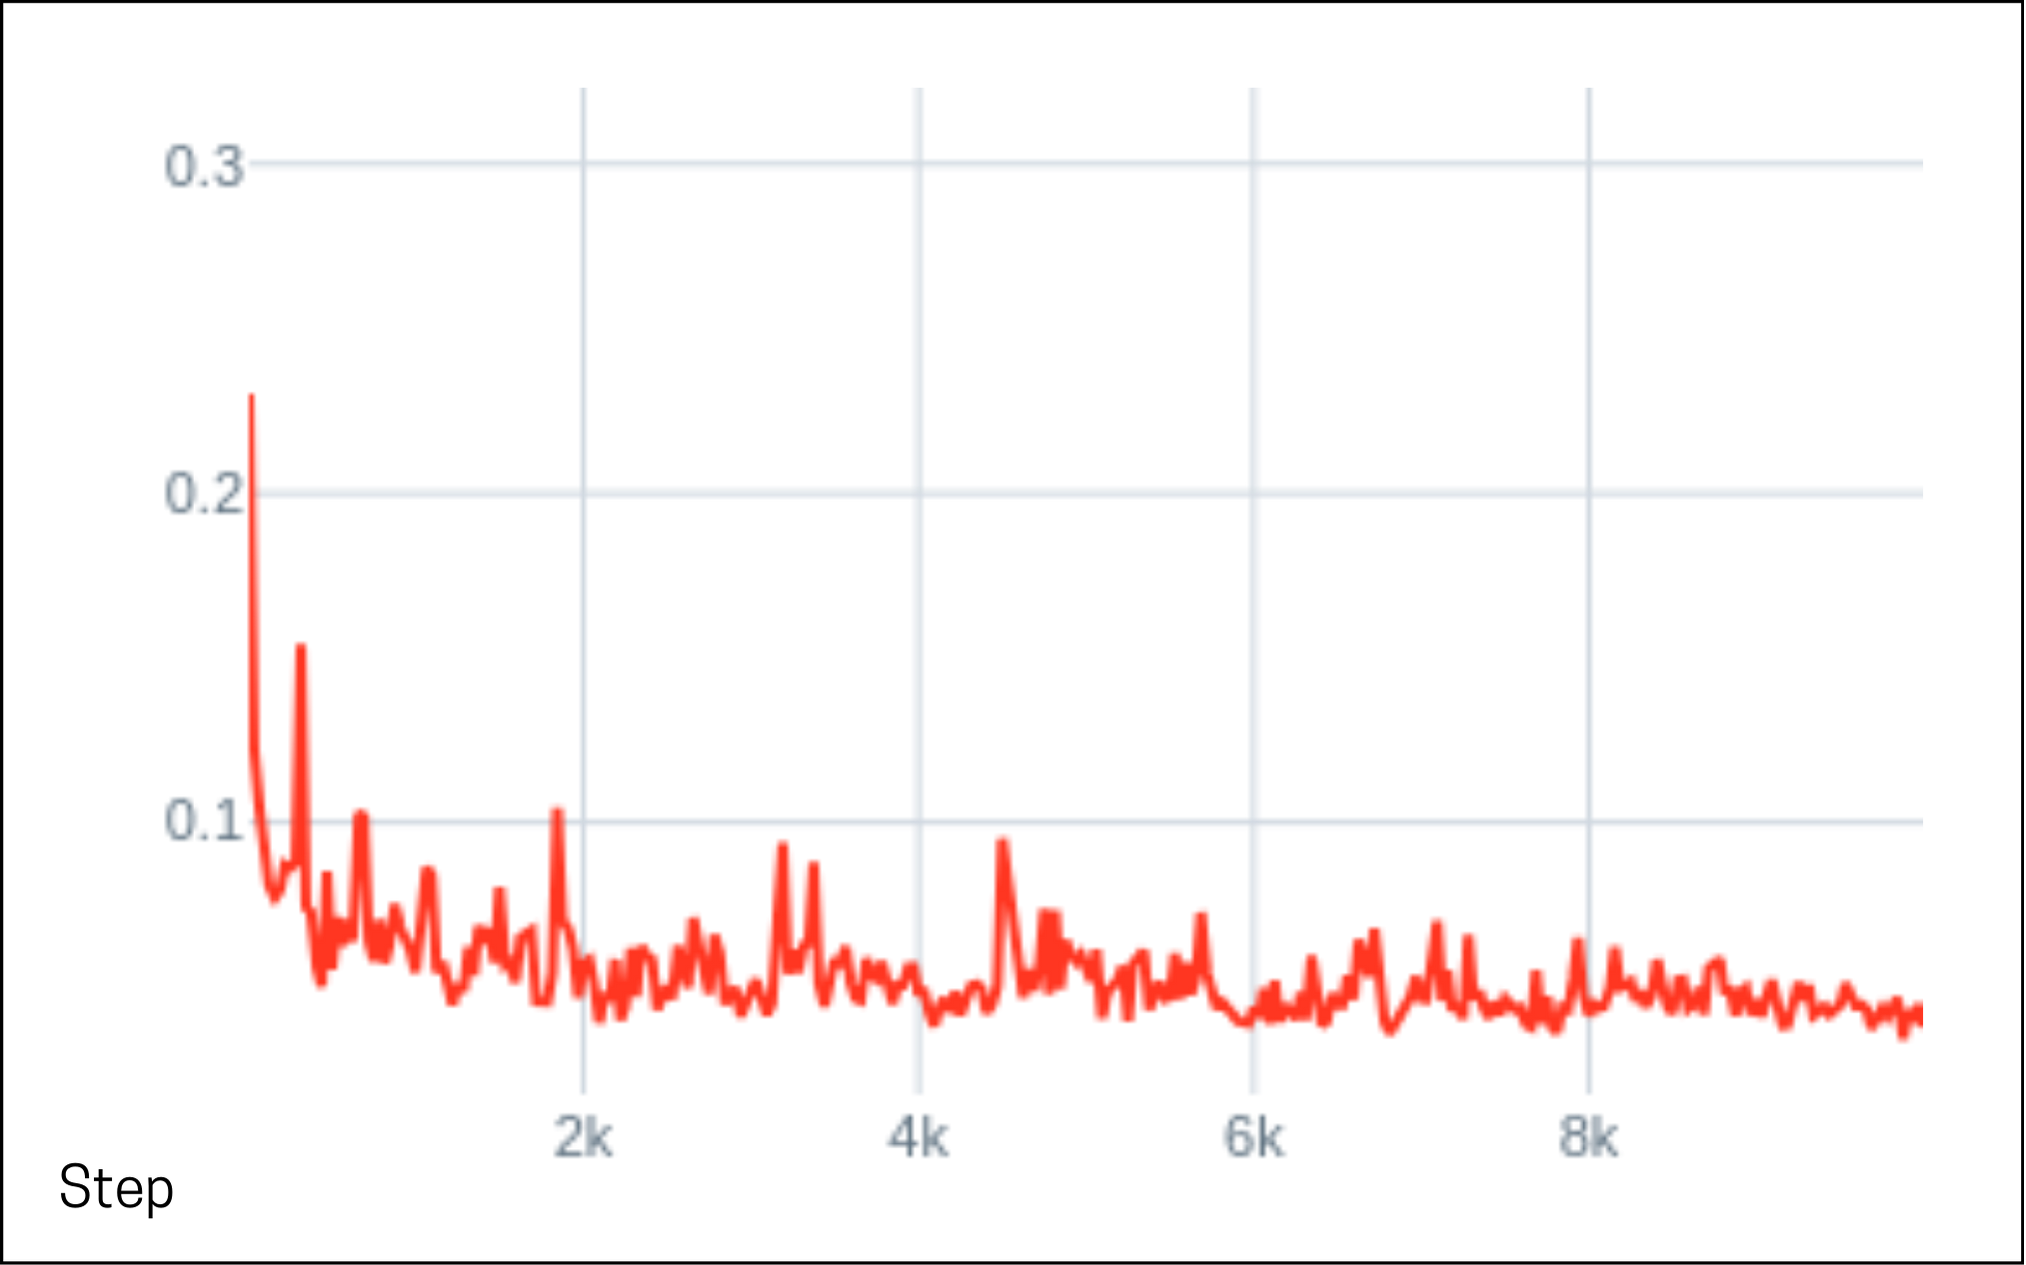
\includegraphics[width=\textwidth]{figures/mean_loss_craft.png}
    \caption{Illustration of the mean loss during CRAFT model training, showing the performance 
    improvement over time. The mean loss decreased rapidly in the first 500 iterations, 
    indicating that the model was able to quickly adapt to the training data. The loss then 
    continued to decrease at a slower rate until around 2,000 iterations, at which point 
    the model's performance began to plateau.}
    \label{fig:mean-loss-craft}
\end{figure}

\subsection{CRAFT Evaluation Metrics}
\label{subsec:craft-evaluation}

Text detection evaluation was performed using precision, recall, and Intersection over Union (IoU) metrics. The CRAFT model demonstrated excellent performance in detecting text regions with high accuracy.

\begin{figure}[H]
    \centering
    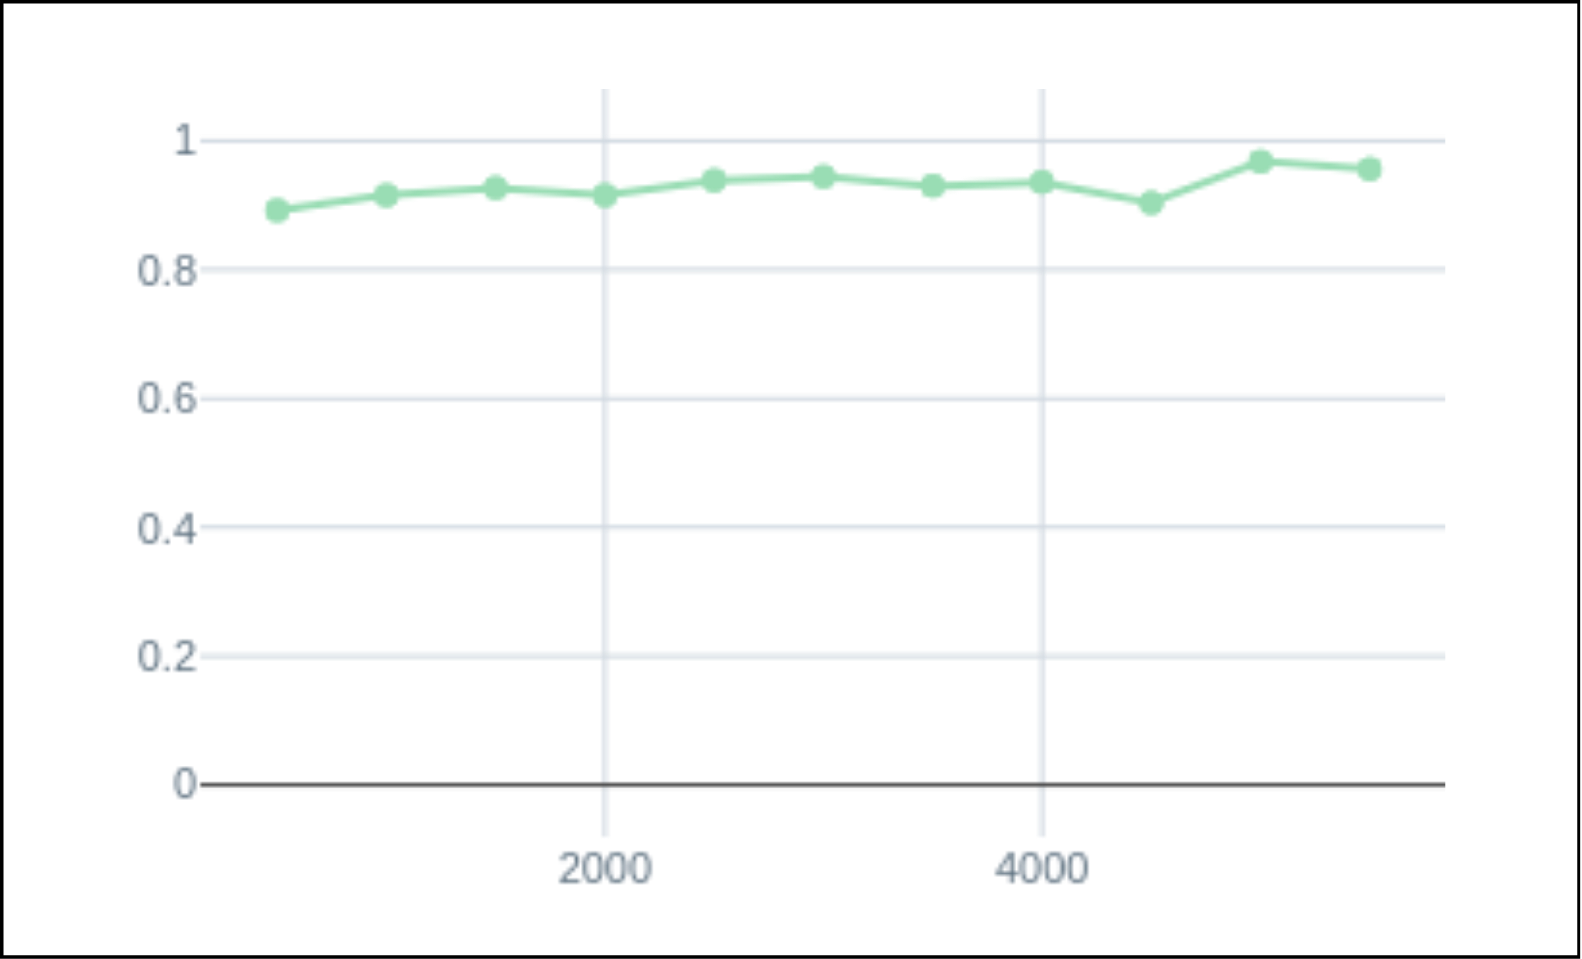
\includegraphics[width=\textwidth]{figures/iou_craft.png}
    \caption{Illustration of the intersection over union (IOU) vs. recall performance of the CRAFT model 
    during text detection evaluation. The IOU is a measure of how well the bounding box predicted 
    by the model overlaps with the ground truth bounding box, while the recall measures how many of 
    the ground truth bounding boxes are detected by the model. The model reaches a high recall of 
    90\% at an IOU of 0.5, indicating that the model is able to detect most of the text regions even 
    when the predicted bounding box is not perfectly aligned with the ground truth.}
    \label{fig:iou-recall-craft}
\end{figure}

The CRAFT model achieved:
\begin{itemize}
\item \textbf{Recall}: 90\% at IoU threshold of 0.5
\item \textbf{Precision}: 89\% 
\item \textbf{F1-score}: 86.8\%
\end{itemize}

These results demonstrate that the model successfully adapted to Khmer script characteristics and can effectively detect text regions in various conditions.

\section{TrOCR for Text Recognition}
\label{sec:trocr-complete}

This section provides a comprehensive examination of the TrOCR (Transformer-based Optical Character Recognition) model implementation, including its architecture, customization for Khmer script, training methodology, and evaluation results.

\subsection{TrOCR Model Architecture}
\label{subsec:trocr-architecture}

For the text recognition component of the pipeline, we used the \textbf{TrOCR} model, a transformer-based OCR system proposed by Microsoft Research. TrOCR stands for \textit{Transformer-based Optical Character Recognition}, and it integrates a vision encoder with a language decoder in a unified encoder-decoder (Seq2Seq) architecture, following the structure of the Vision Transformer (ViT) and pre-trained language models like BART.

The TrOCR model takes the cropped text-line image detected by CRAFT and processes it through a \textbf{ViT-based encoder}, which extracts rich visual features. These features are then passed to the \textbf{transformer decoder}, which generates the text sequence token-by-token, using cross-attention to focus on relevant image features while decoding. This allows the model to handle complex scripts like Khmer with better accuracy and context-awareness.

\begin{figure}[H]
    \centering
    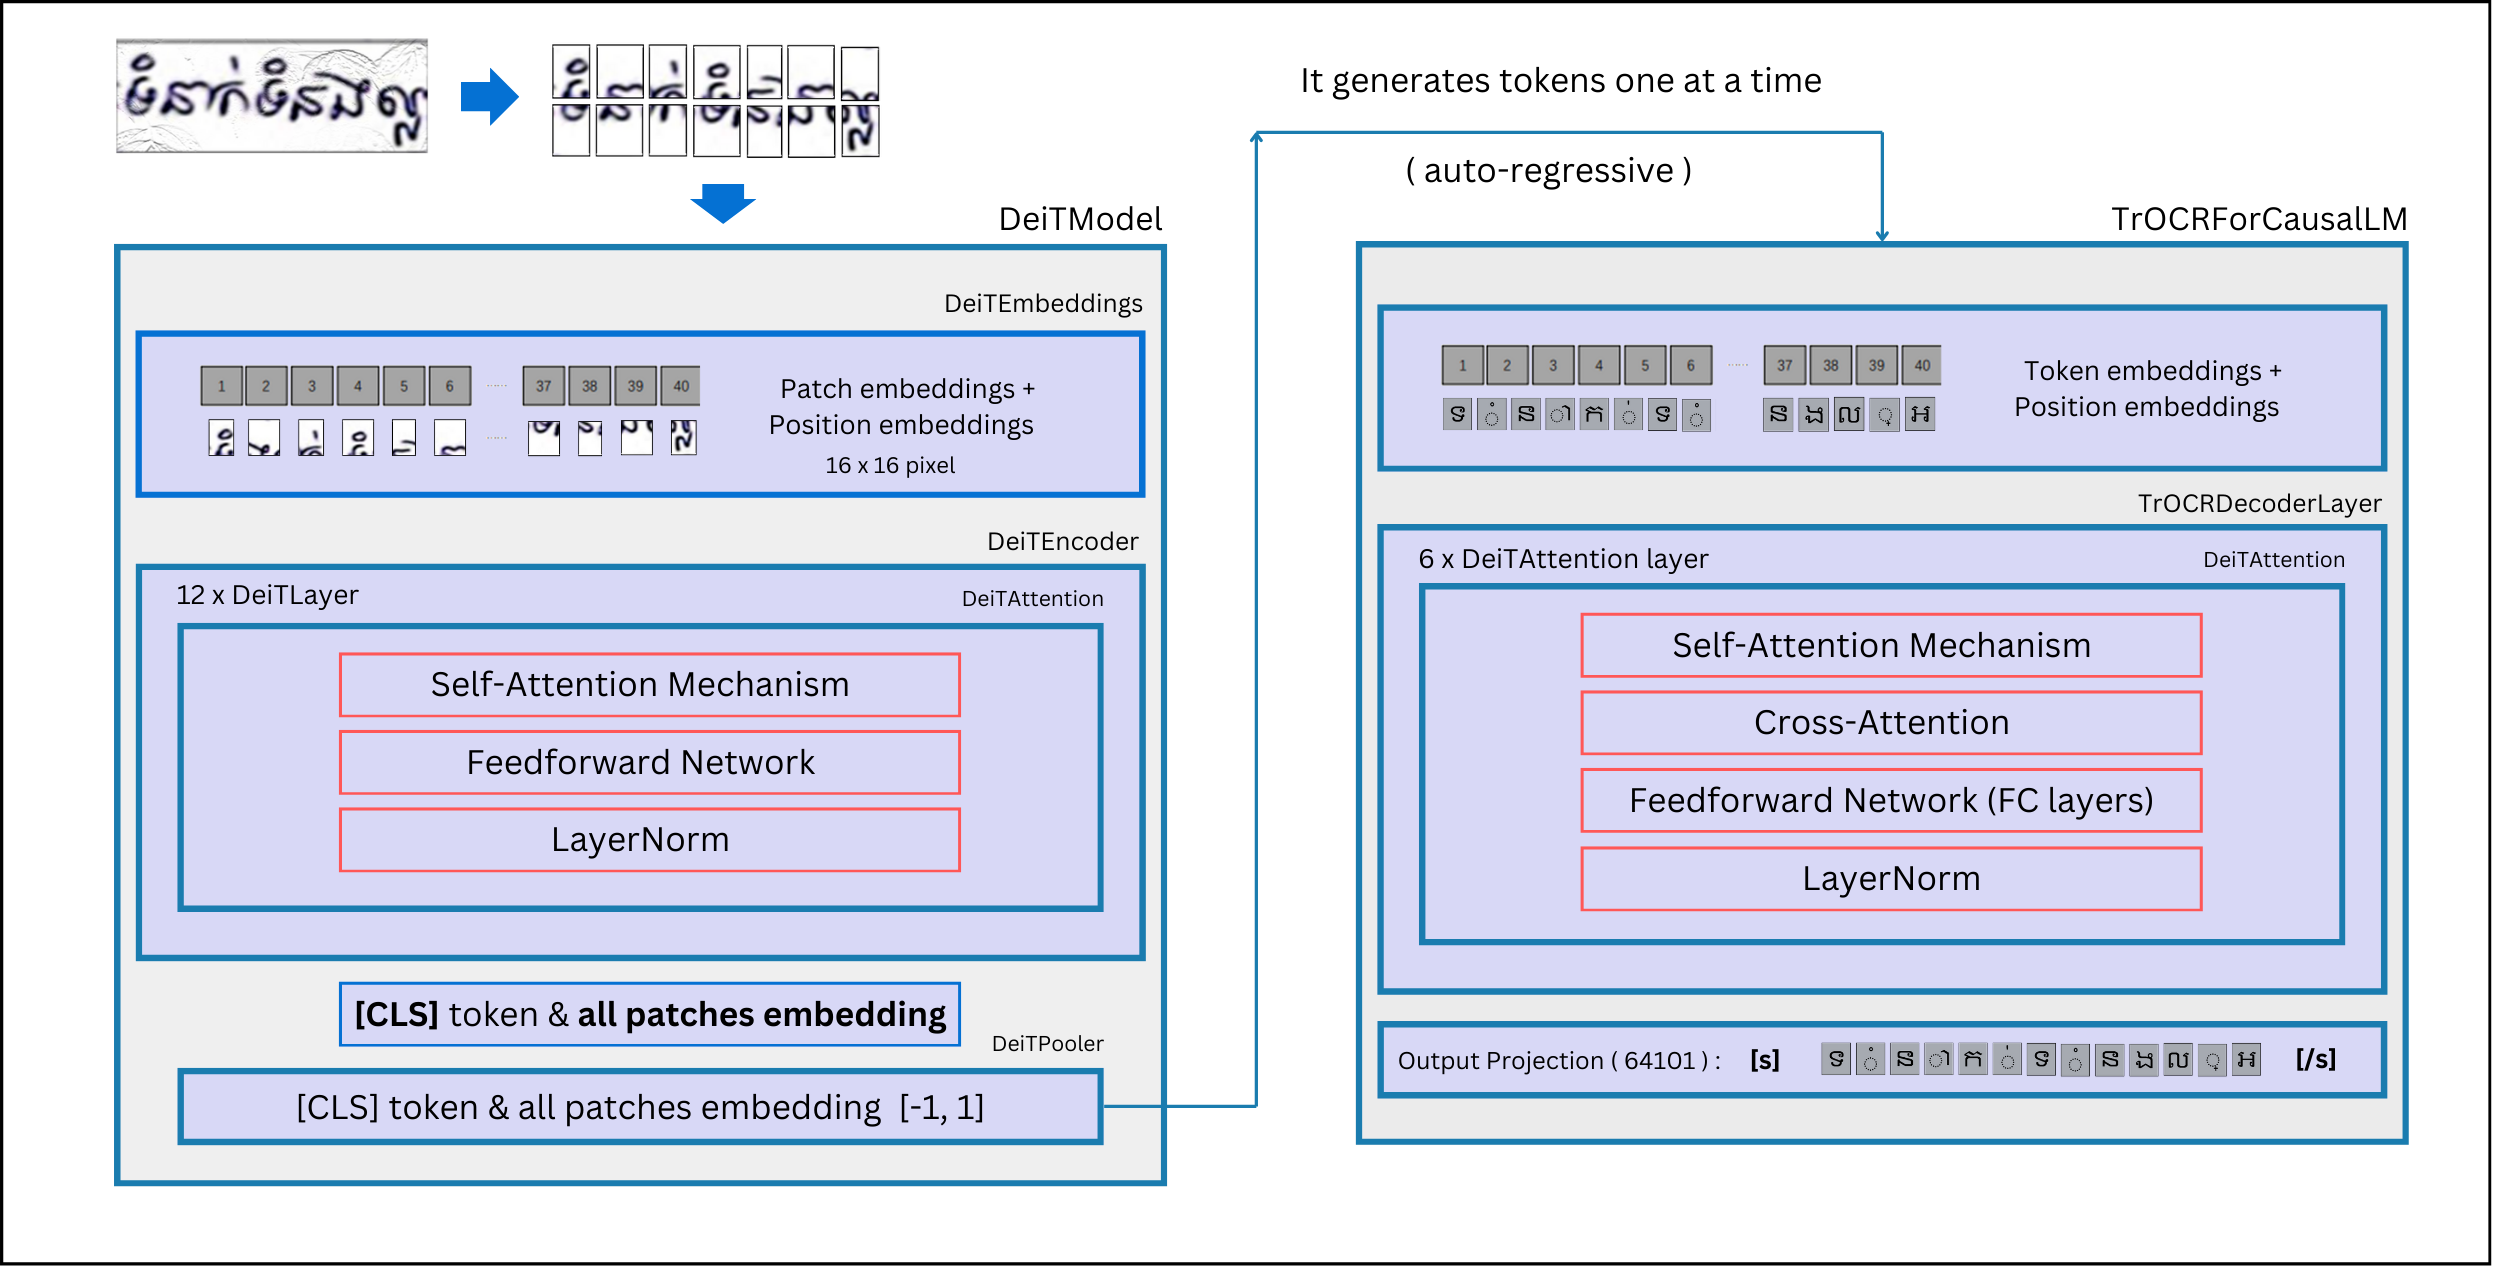
\includegraphics[width=\textwidth]{figures/trocr_model.png}
    \caption{Illustration of the TrOCR model architecture used for text recognition.}
    \label{fig:trocr-model}
\end{figure}

\subsection{Custom Khmer Processor Development}
\label{subsec:trocr-customization}

To make the TrOCR model understand Khmer tokens, we customized the processor without modifying the original model architecture. We developed a CustomKhmerTokenizer based on a predefined list of unique Khmer and English characters, including special tokens such as \textit{<s>}, \textit{</s>}, and \textit{<pad>}, to handle the encoding of text into token IDs and the decoding of token IDs back into readable text.

This tokenizer was then wrapped inside a custom processor that mimics the behavior of Hugging Face's TrOCRProcessor, allowing seamless integration with TrOCR's image processing pipeline. By doing so, we enabled the model to work with Khmer script during both training and inference, while preserving the original TrOCR model's structure and leveraging its pretrained capabilities.

\begin{figure}[H]
    \centering
    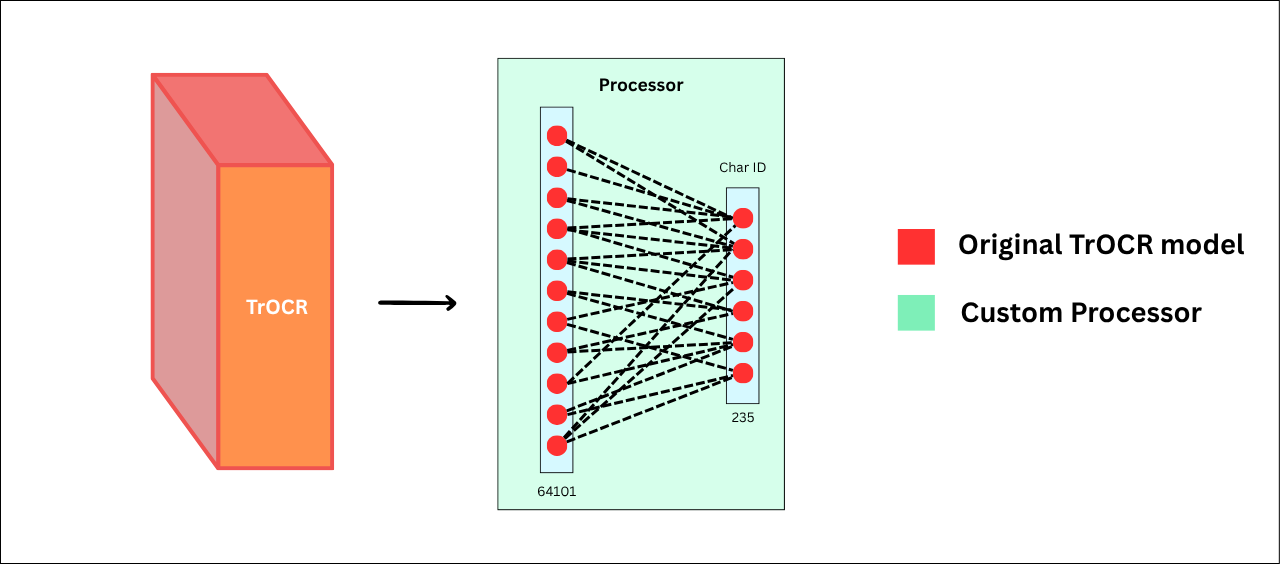
\includegraphics[width=\textwidth]{figures/Customize_processor.png}
    \caption{Architecture of the customized TrOCR pipeline. 
    The original TrOCR model is extended with a custom processor, 
    which includes two additional fully connected layers 
    (FC1 and FC2) tailored for Khmer character decoding.}
    \label{fig:trocr-custom-processor}
\end{figure}

\subsection{TrOCR Dataset and Training Methodology}
\label{subsec:trocr-training}

For the TrOCR model, we selected the base model because we were working with a multilingual dataset and wanted the model to have sufficient parameter capacity for this task. The training dataset consisted of 3.5 million synthetic images generated using our text-to-image pipeline.

\begin{figure}[H]
    \centering
    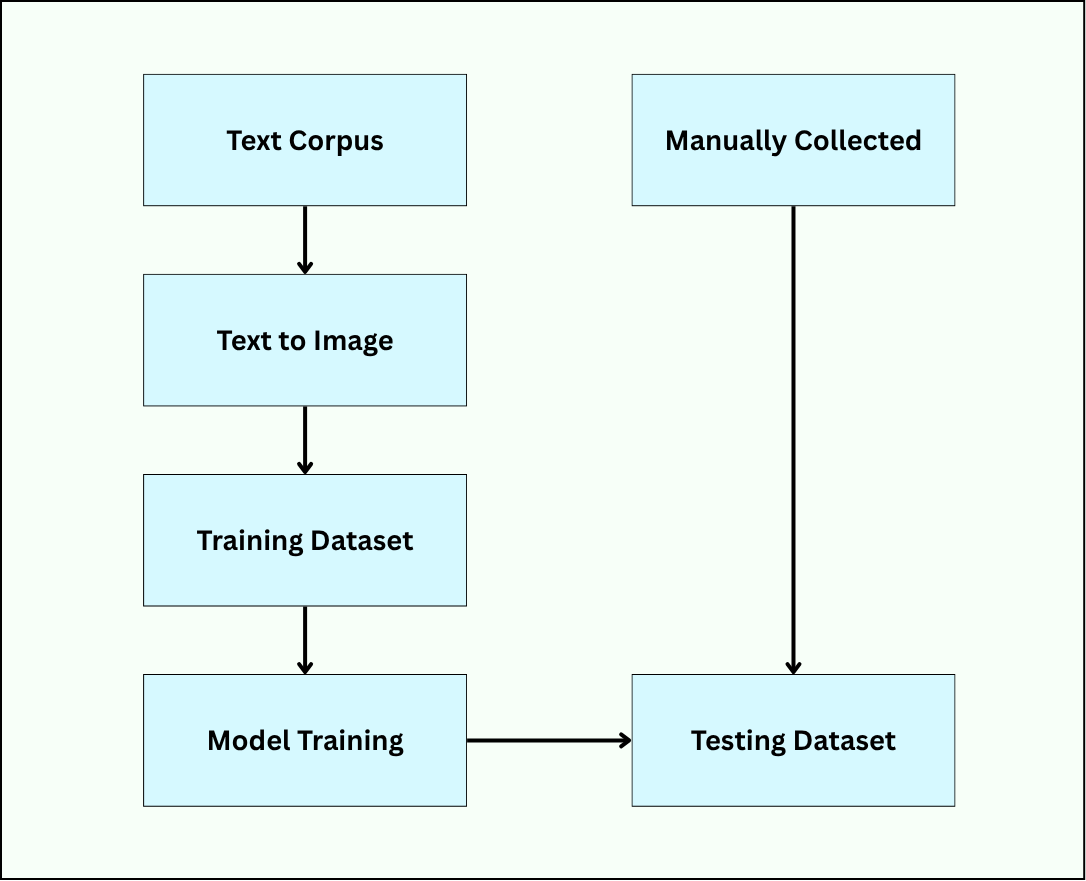
\includegraphics[width=\textwidth]{figures/trocr_model_overflow_training.png}
    \caption{Overview of the TrOCR training process. Text-generated 
    images form the training set, while real-world samples are 
    manually collected for testing and evaluation.}
    \label{fig:trocr-training-pipeline}
\end{figure}

After experimenting with different hyperparameters, we found the optimal configuration:
\begin{itemize}
\item \textbf{Batch size}: 1024
\item \textbf{Learning rate}: 0.0001
\item \textbf{Epochs}: 2
\item \textbf{Dataset size}: 3.5 million images
\end{itemize}

The choice of batch size 1024 was crucial for model generalization. Initial experiments with smaller batch sizes (8, 16, 32, 128, 256) resulted in severe overfitting, as demonstrated in Figure~\ref{fig:trocr-overfitting}.

\subsection{TrOCR Training Results and Performance}
\label{subsec:trocr-training-results}

\begin{figure}[H]
    \centering
    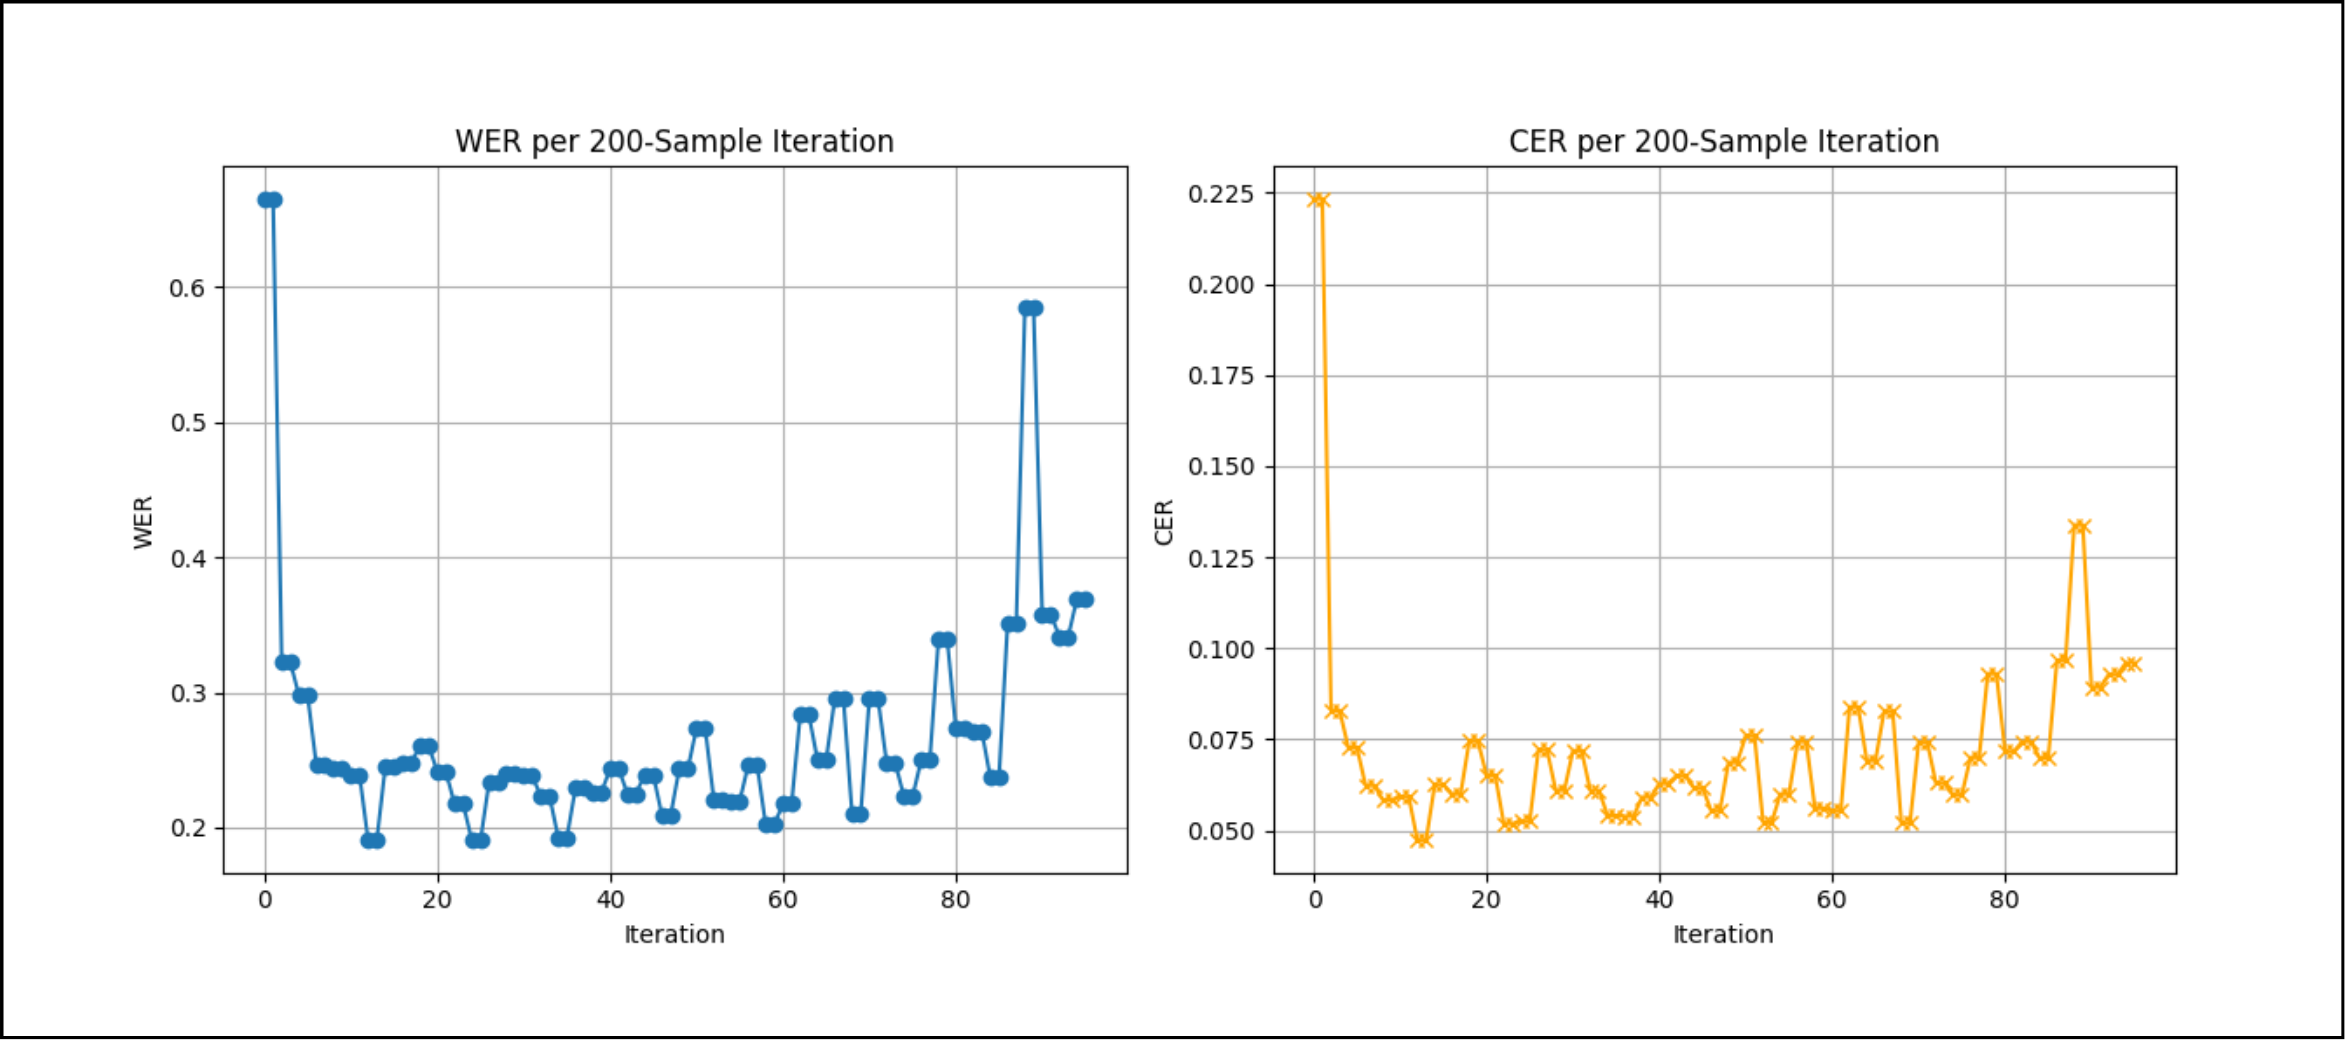
\includegraphics[width=\textwidth]{figures/trocr_overfitting_v1.png}
    \caption{Training and validation loss curves for TrOCR model with batch size 8, 
    clearly showing overfitting behavior where training loss decreases while validation loss increases.}
    \label{fig:trocr-overfitting}
\end{figure}

The graph above illustrates a clear case of overfitting when using a batch size of 8. The training loss continues to decrease while the validation loss starts to increase, indicating that the model learns very specific patterns from the training data rather than generalizing well to unseen data.

\begin{figure}[H]
    \centering
    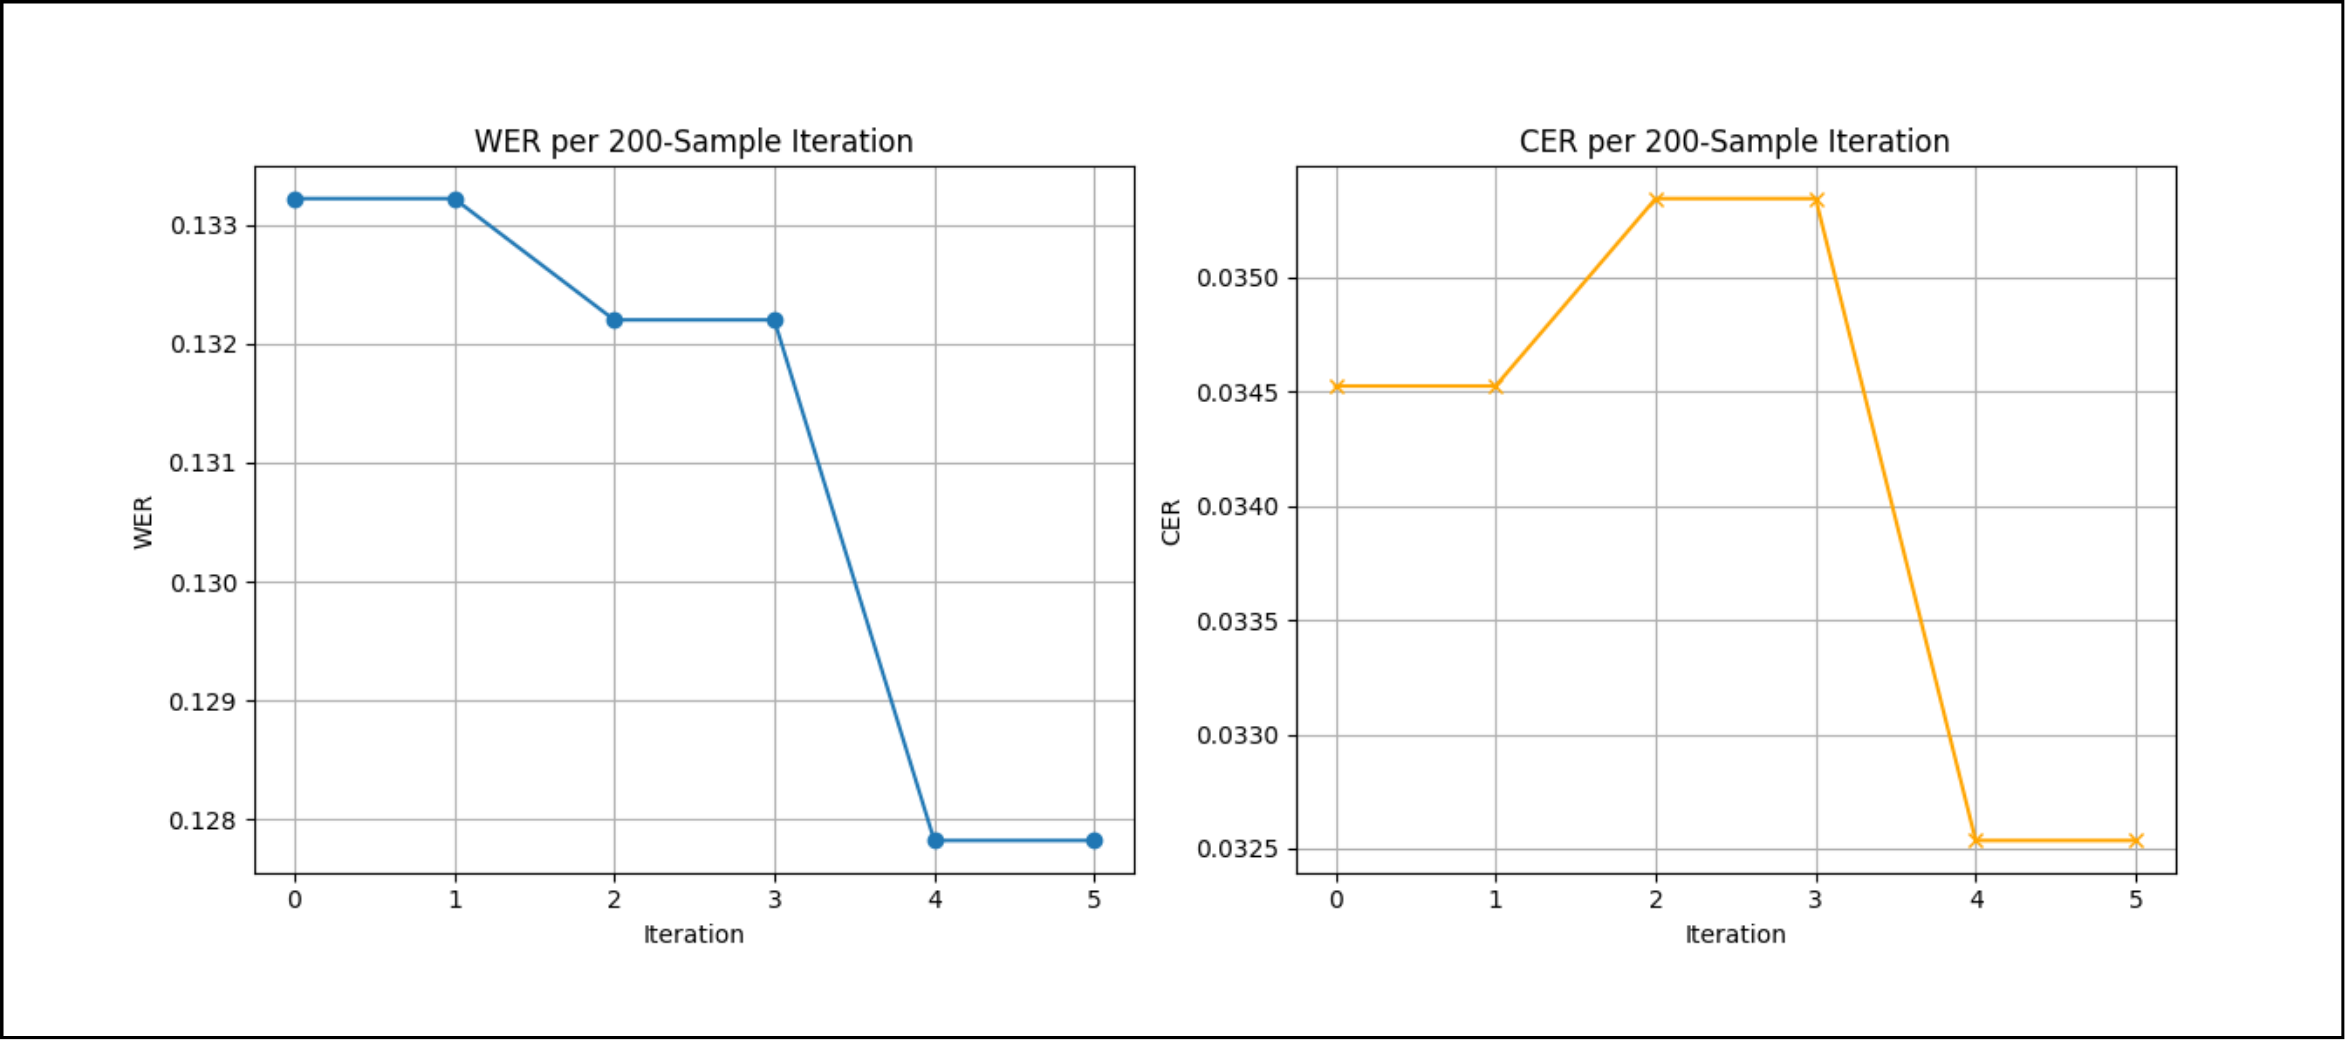
\includegraphics[width=\textwidth]{figures/trocr_fine_tuning.png}
    \caption{Training and validation metrics for TrOCR model with batch size 1024, 
    showing Character Error Rate (CER) and Word Error Rate (WER) over training steps. 
    The model demonstrates excellent performance from early training steps, with CER quickly 
    reaching around 0.03 and WER staying below 0.12.}
    \label{fig:trocr-fine-tuning}
\end{figure}

With the optimized batch size of 1024, the model showed remarkable performance from early stages of training, with CER quickly stabilizing around 0.03 and WER maintaining values below 0.12. This rapid convergence can be attributed to the utilization of pretrained weights and the larger batch size enabling better generalization.

\subsection{TrOCR Evaluation Metrics}
\label{subsec:trocr-evaluation}

For evaluating the text recognition performance of our TrOCR model, we employed three key metrics: Character Error Rate (CER), Word Error Rate (WER), and Accuracy. These metrics provide a comprehensive assessment of the model's recognition capabilities.

\subsubsection{Character Error Rate (CER)}
\label{subsubsec:cer-metric}

Character Error Rate (CER) measures the ratio of incorrect characters to the total number of characters in the ground truth text. It is calculated as:

\begin{equation}
    CER = \frac{S + D + I}{N}
\end{equation}

where $S$ is the number of substitutions, $D$ is the number of deletions, $I$ is the number of insertions, and $N$ is the total number of characters in the ground truth text.

\subsubsection{Word Error Rate (WER)}
\label{subsubsec:wer-metric}

Word Error Rate (WER) operates at the word level, measuring the ratio of incorrect words to the total number of words in the ground truth text. WER is calculated as:

\begin{equation}
    WER = \frac{S_w + D_w + I_w}{N_w}
\end{equation}

where $S_w$ is the number of word substitutions, $D_w$ is the number of word deletions, $I_w$ is the number of word insertions, and $N_w$ is the total number of words in the ground truth text.

\subsubsection{Accuracy Metrics}
\label{subsubsec:accuracy-metric}

Accuracy is the complement of the error rate, representing the percentage of correctly recognized characters or words. For character-level accuracy:

\begin{equation}
    Accuracy_{char} = 1 - CER
\end{equation}

And for word-level accuracy:

\begin{equation}
    Accuracy_{word} = 1 - WER
\end{equation}

The final TrOCR model achieved:
\begin{itemize}
\item \textbf{Overall CER}: 0.02
\item \textbf{Khmer CER}: 0.04
\item \textbf{English CER}: 0.01
\item \textbf{Mixed-language CER}: 0.06
\end{itemize}

\section{End-to-End OCR Pipeline}
\label{sec:end-to-end-pipeline}

This section describes the integration of CRAFT and TrOCR models into a unified end-to-end OCR system capable of processing multilingual documents containing both Khmer and English text.

\subsection{Pipeline Architecture}
\label{subsec:pipeline-architecture}

The overall workflow is presented in Figure~\ref{fig:trocr-inference-full-pipeline}. The pipeline begins with input images containing English and Khmer text, or mixed-language content. The preprocessing step converts images to grayscale to streamline downstream processing and improve model prediction accuracy.

\begin{figure}[H]
    \centering
    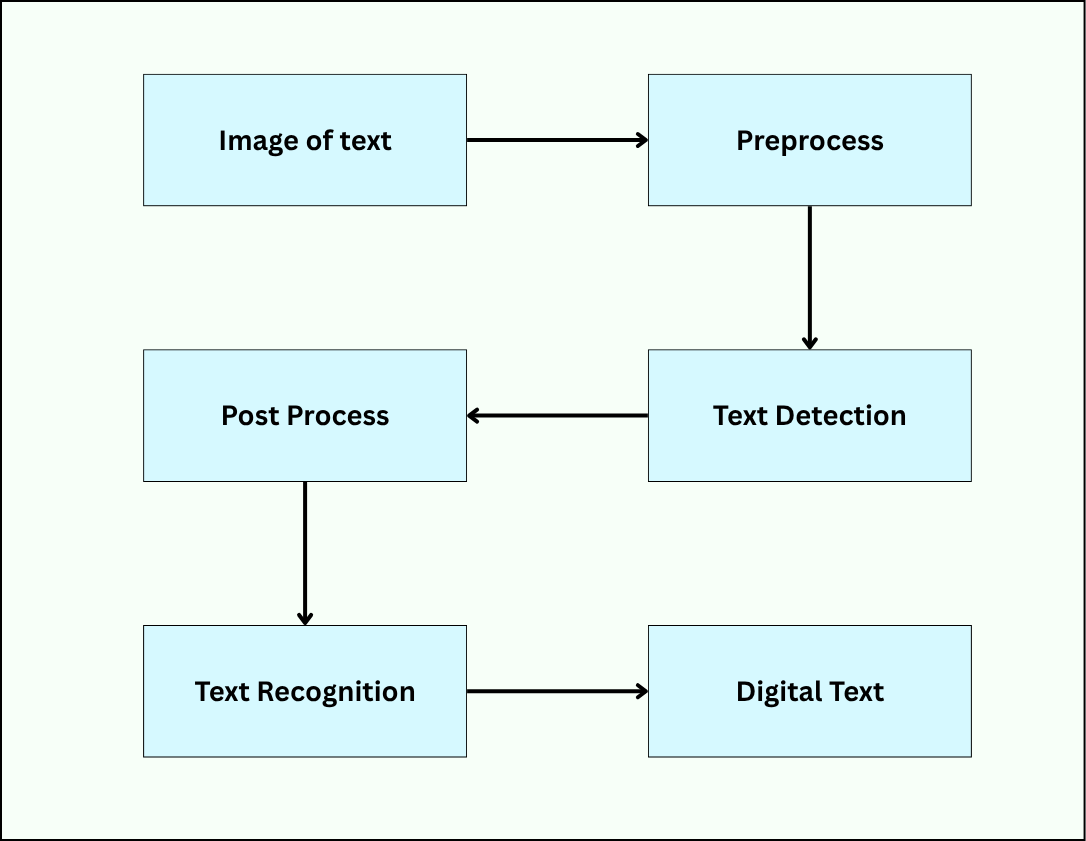
\includegraphics[width=\textwidth]{figures/khmerOCR_inference_full_pipeline.png}
    \caption{End-to-end OCR inference pipeline for converting text images into digital text.}
    \label{fig:trocr-inference-full-pipeline}
\end{figure}

\subsection{Pipeline Processing Steps}
\label{subsec:pipeline-steps}

The complete pipeline operates through the following sequential steps:

\begin{enumerate}
\item \textbf{Image Preprocessing}: Input images are converted to grayscale and normalized to ensure consistent processing across different image types and qualities.

\item \textbf{Text Detection}: The CRAFT model detects text regions in the image on a text-line basis, generating bounding boxes for each detected text segment.

\item \textbf{Post-processing and Reordering}: Detected text-lines undergo post-processing to ensure correct reading order, accounting for document layout and text flow patterns.

\item \textbf{Text-line Cropping}: Individual text-line regions are extracted from the original image based on CRAFT detection results.

\item \textbf{Text Recognition}: Each cropped text-line image is processed by the TrOCR model to generate the corresponding digital text output.

\item \textbf{Output Assembly}: Recognized text from all text-lines is assembled in the correct order to produce the final digital document.
\end{enumerate}

\subsection{Pipeline Integration Benefits}
\label{subsec:pipeline-benefits}

The integration of CRAFT and TrOCR provides several advantages:

\begin{itemize}
\item \textbf{Character-level Detection}: CRAFT's character-aware detection is particularly effective for complex scripts like Khmer with stacked characters and diacritics.

\item \textbf{Transformer-based Recognition}: TrOCR's attention mechanism allows for better context understanding and improved accuracy on both Khmer and English text.

\item \textbf{Multilingual Support}: The pipeline seamlessly handles documents containing both Khmer and English text without requiring language-specific preprocessing.

\item \textbf{End-to-end Processing}: The unified pipeline eliminates the need for manual intervention between detection and recognition stages.
\end{itemize}

This comprehensive approach ensures robust performance across diverse document types and text conditions, making it suitable for real-world OCR applications in multilingual environments.